Although relatively radiation tolerant, lead tungstate scintillating crystals do lower the light output when exposed to radiation and recover when the radiation source is removed, trough spontaneus thermal-annealing mechanisms. Extensive studies performed at the Institute for High Energy Physics (IHEP) in Protvino, Russia, confirmed that the PbWO$_4$ light output changes with the irradiation dose rate. In particular, dedicated measurements showed that degradation of light output in PbWO$_4$ crystals occurs due to light transmission loss only, rather than changes in the intrinsic scintillation mechanism \cite{1}. Further complications arise because at the same irradiation intensity, changes in light output may vary from one crystal to another \cite{2} \cite{3}. \textcolor{red}{Add plot of radiation damage measurement here - and quote S.Fegan paper? Probably yes, since it also shows the effect of light annealing}

\begin{figure}[ht!]
\centering
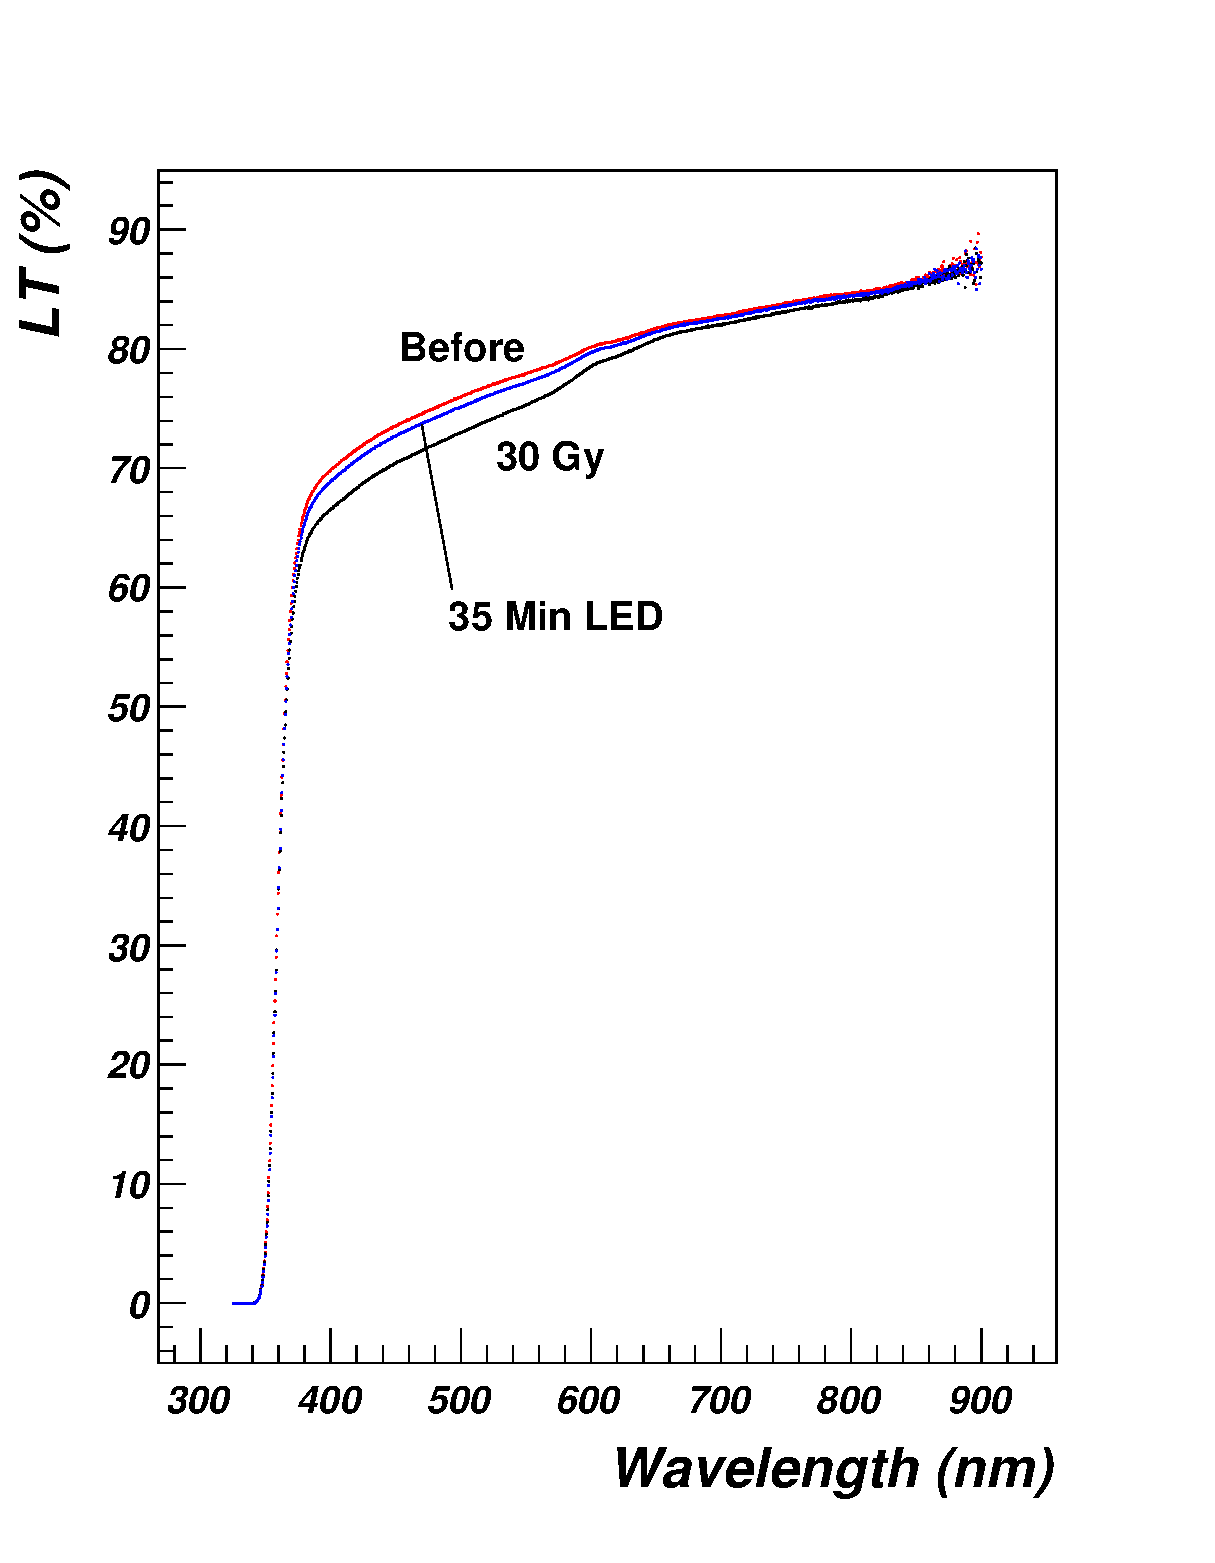
\includegraphics[width=0.60\textwidth]{LT_CrystalHPS_rec.eps}
\caption{A schematic view of an ECal module.}
\label{CrystalRadDamage}
\end{figure}
 


In order to preserve the intrinsic ECal energy resolution, the response of the crystals has to  be continuously monitored and, if necessary, recalibrated. To this end, a custom, LED-based monitoring system was specifically designed and installed in the detector setup after the 2012 test run. With this system, a light pulse, with variable amplitude and width, can be injected independently in each crystal. The pulse is emitted by a red/blue bi-color LED placed in front of the crystal.
By measuring the response of the whole chain (crystal + APD + amplifier) to the pulse, any variation in the channel response can be acknowledged and, if necessary, corrected. Furthermore, since radiation damage in the PbWO$_4$ crystals is not uniform over the transmission spectrum, but is mostly concentrated in the blue region (up to $\simeq$ 500 nm), the use of a red/blue bi-color LED can also help in determining which component in the chain is responsible of a possible channel response variation. Given the possibility to turn on one or more channels at time, with a programmable pattern, such a system has been extensively used during the Ecal and trigger commissioning. Finally, studies are currently undergoing on the possibility to use the monitoring system to recover crystals radiation damage trough a light annealing mechanism. \textcolor{red}{CITATION NEEDED}

The LED monitoring system setup is as follows. Each LED is hosted in a PEEK plastic holder placed in front of the crystal, with a proper light collimation hole. LEDs are connected trough twisted-pair wires to 4 printed-circuit boards - two for Ecal top, two for Ecal bottom - that, in turns, are connected to 8 driver circuits, mounted directly on top and on bottom of the detector external enclosure. The drivers host the electronic circuits used to pilote the LEDs, and have them producing the light pulses, with programmable amplitude, width and frequency. Drivers communicate with the main system controller via I$^2$C protocol. The controller, that also provides power and the master clock to the drivers, hosts a PIC32-based board, with a custom firmware, connected trough Ethernet to the HPS slow-controls network.
 \textcolor{red}{More details?} 


%\bibitem{1} V.A. Batarin, et al., Nucl. Instr. and Meth. A 540 (2005) 131 (e-Print
%ArXiv physics/0410133).
%\bibitem{2} V.A. Batarin, et al., Nucl. Instr. and Meth. A 512 (2003) 484 (e-Print
%ArXiv hep-ex/0210011).
%\bibitem{3} V.A. Batarin, et al., Nucl. Instr. and Meth. A 550 (2005) 543 (e-Print
%ArXiv physics/0504085).
